\subsection{Addressing}
\label{sec:p2p:addressing}

Each node possesses an ECDSA public key which acts as a unique identifier in the netork. The identifier is structured using \href{https://github.com/multiformats/multiformats}{multiformats} by Protocol Labs and encoded using \href{https://en.bitcoin.it/wiki/Base58Check_encoding}{Base58} encoding, known from Bitcoin. This leads to the multiformats prefix \textsf{0x002508021221} which is concatenated to the compressed ECDSA public key, yielding an identifier $id$ of 39 bytes and a string representation given by

\begin{center}
    $id = base58.encode(\mathsf{0x002508021221} \ || \ \mathsf{pubKey})$
\end{center}

Identifiers distinguish nodes from each other, whereas addresses allow nodes to establish a connection to each other. HOPR distinguishes two types of addresses: \textit{direct addresses} and \textit{relay addresses}. Both address types are structured using the \href{https://github.com/multiformats/multiaddr}{multiaddr} standard by Protocol Labs.

\paragraph{Direct Addresses}

Nodes that are able to gain control over a TCP socket can have one or more direct address which are determined by their network adapter. The addresses include the loopback IP address, e.g. \textsf{127.0.0.1}, the local IP address, e.g. \textsf{192.168.0.2} as well as, if available, the public IP address, e.g. \textsf{1.2.3.4}. A node with identifier $id$ and public IP address \textsf{1.2.3.4} listening to TCP port $9091$ has the addr

\begin{center}
    $addr = \mathsf{/ip4/1.2.3.4/tcp/9091/}\text{\textless$id$\textgreater{}}$
\end{center}

\paragraph{Relay Addresses}

Due to security concern and the scarcity of IPv4 addresses, many consumer routers hide connected nodes behind a NAT, such that other nodes have a hard time establishing a direct connection to these nodes. To solve this issue, nodes keep a connection to selected relay nodes and publish \textit{relay addresses} to tell others who want to establish a direct connection which relay node to connect if they cannot reach them directly. Once the relayed connection has been established, nodes can exchange signalling information and determine how to connect directly.

\begin{figure}[H]
    \centering
    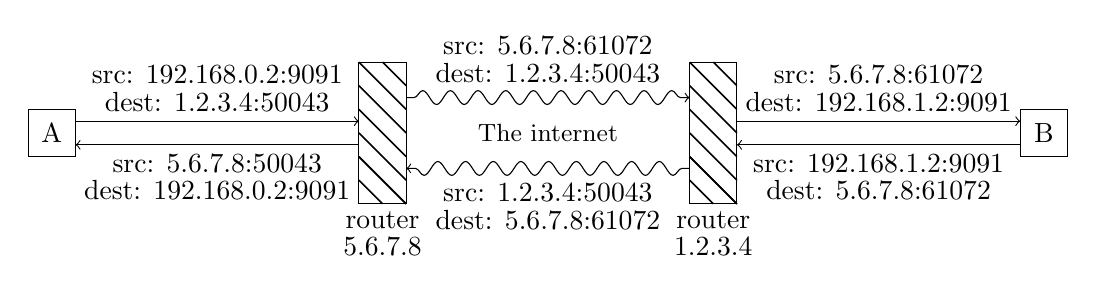
\begin{tikzpicture}
        \def\nodeWidth{0.6}
        \def\nodeHeight{0.6}
        \def\routerWidth{0.6}
        \def\routerHeight{1.8}
        \def\routerOffset{4.2}

        % Subnet A
        \draw (0,0) rectangle (\nodeWidth,\nodeHeight) node[midway] {A};

        % Interaction with router A
        \draw[->] (\nodeWidth,0.75*\nodeHeight) -- (\routerOffset,0.75*\nodeHeight) node[midway,above] {\smaller{\shortstack{src: 192.168.0.2:9091\\dest: 1.2.3.4:50043}}};

        \draw[->] (\routerOffset,0.25*\nodeHeight) -- (\nodeWidth,0.25*\nodeHeight) node[midway,below] {\smaller{\shortstack{src: 5.6.7.8:50043\\dest: 192.168.0.2:9091}}};

        % Router to router interaction
        \begin{scope}[shift={(0,-0.6)}]
            \draw[->,decorate,decoration={snake,pre length=1mm,post length=1mm}] (\routerOffset+\routerWidth,0.75*\routerHeight) -- (2*\routerOffset,0.75*\routerHeight) node[midway,above=2pt] {\smaller{\shortstack{src: 5.6.7.8:61072\\dest: 1.2.3.4:50043}}};
            \draw[->,decorate,decoration={snake,pre length=1mm,post length=1mm}] (2*\routerOffset,0.25*\routerHeight) -- (\routerOffset+\routerWidth,0.25*\routerHeight) node[midway,below=2pt] {\smaller{\shortstack{src: 1.2.3.4:50043\\dest: 5.6.7.8:61072}}};

            \path (\routerOffset+\routerWidth,0.5*\routerHeight) -- (2*\routerOffset,0.5*\routerHeight) node[midway] {\small{The internet}};
        \end{scope}

        % Subnet B
        \begin{scope}[shift={(3*\routerOffset,0)}]
            \draw (0,0) rectangle (\nodeWidth,\nodeHeight) node[midway] {B};
            % Interaction with router B
            \draw[->] (-\routerOffset+\routerWidth,0.75*\nodeHeight) -- (0,0.75*\nodeHeight) node[midway,above] {\smaller{\shortstack{src: 5.6.7.8:61072\\dest: 192.168.1.2:9091}}};

            \draw[->] (0,0.25*\nodeHeight) -- (-\routerOffset+\routerWidth,0.25*\nodeHeight) node[midway,below] {\smaller{\shortstack{src: 192.168.1.2:9091\\dest: 5.6.7.8:61072}}};
        \end{scope}

        \foreach \offset\name\address in{1/A/5.6.7.8,2/B/1.2.3.4} {
                \begin{scope}[shift={(\offset*\routerOffset,-0.6)}]
                    \def\a{0.6}
                    \def\b{1.8}
                    \def\diff{1.2}

                    \def\lw{0.2}

                    \foreach \x [count=\i] in{0,0.3,0.6,...,\a}{
                            \draw [line width=\lw mm](\x,0)--(0,\x) (\x,\b)--(\a,\b-\a+\x);
                        }
                    \foreach \x [count=\i] in{0,0.3,0.6,...,\diff}{
                            \draw [line width=\lw mm](0,\a+\x)--(\a,\x);
                        }
                    \draw (0,0) rectangle  node[below=25pt] {\smaller{\shortstack{router\\\address}}} (\routerWidth,\routerHeight);
                \end{scope}

            }
    \end{tikzpicture}
    \label{fig:successful-nat-traversal}
    \caption{Successful NAT traversal between A, running on 192.168.0.2, and B, running on 192.168.1.2, after exchanging signalling information.}
\end{figure}

A relay address includes the identifier $relayId$ of the relay to which the node need to connect first and the identifier $id$ of the final destination.

\begin{center}
    \textsf{/p2p/}\textless\textsf{$relayId$}\textgreater\textsf{/p2p-circuit/p2p/}\textless{}\textsf{$id$}\textgreater{}
\end{center}

Relay nodes come with a limited capacity of relay slots and depending on the geographical proximity, it becomes clear that some relay nodes suit better than other. Hence, at startup, each node first retrieves a list of potential relay nodes, see \lcnameref{sec:p2p:peer-discovery} for more information, and tries to register a relay slot with the most promising ones and announces the list of relay addresses in the network.

Hence, whenever another node is unable to connect directly, it first connects to one of the published relay nodes and asks them to extend the connection to the intended node.